\documentclass[10pt,a4paper]{article}\usepackage[]{graphicx}\usepackage[]{color}
%% maxwidth is the original width if it is less than linewidth
%% otherwise use linewidth (to make sure the graphics do not exceed the margin)
\makeatletter
\def\maxwidth{ %
  \ifdim\Gin@nat@width>\linewidth
    \linewidth
  \else
    \Gin@nat@width
  \fi
}
\makeatother

\definecolor{fgcolor}{rgb}{0.345, 0.345, 0.345}
\newcommand{\hlnum}[1]{\textcolor[rgb]{0.686,0.059,0.569}{#1}}%
\newcommand{\hlstr}[1]{\textcolor[rgb]{0.192,0.494,0.8}{#1}}%
\newcommand{\hlcom}[1]{\textcolor[rgb]{0.678,0.584,0.686}{\textit{#1}}}%
\newcommand{\hlopt}[1]{\textcolor[rgb]{0,0,0}{#1}}%
\newcommand{\hlstd}[1]{\textcolor[rgb]{0.345,0.345,0.345}{#1}}%
\newcommand{\hlkwa}[1]{\textcolor[rgb]{0.161,0.373,0.58}{\textbf{#1}}}%
\newcommand{\hlkwb}[1]{\textcolor[rgb]{0.69,0.353,0.396}{#1}}%
\newcommand{\hlkwc}[1]{\textcolor[rgb]{0.333,0.667,0.333}{#1}}%
\newcommand{\hlkwd}[1]{\textcolor[rgb]{0.737,0.353,0.396}{\textbf{#1}}}%
\let\hlipl\hlkwb

\usepackage{framed}
\makeatletter
\newenvironment{kframe}{%
 \def\at@end@of@kframe{}%
 \ifinner\ifhmode%
  \def\at@end@of@kframe{\end{minipage}}%
  \begin{minipage}{\columnwidth}%
 \fi\fi%
 \def\FrameCommand##1{\hskip\@totalleftmargin \hskip-\fboxsep
 \colorbox{shadecolor}{##1}\hskip-\fboxsep
     % There is no \\@totalrightmargin, so:
     \hskip-\linewidth \hskip-\@totalleftmargin \hskip\columnwidth}%
 \MakeFramed {\advance\hsize-\width
   \@totalleftmargin\z@ \linewidth\hsize
   \@setminipage}}%
 {\par\unskip\endMakeFramed%
 \at@end@of@kframe}
\makeatother

\definecolor{shadecolor}{rgb}{.97, .97, .97}
\definecolor{messagecolor}{rgb}{0, 0, 0}
\definecolor{warningcolor}{rgb}{1, 0, 1}
\definecolor{errorcolor}{rgb}{1, 0, 0}
\newenvironment{knitrout}{}{} % an empty environment to be redefined in TeX

\usepackage{alltt}
\usepackage[utf8]{inputenc}
\usepackage[ngerman]{babel}
\usepackage{amsmath}
\usepackage{amsfonts}
\usepackage{amssymb}
\usepackage{graphicx}
\usepackage{natbib}
\usepackage{float}
\usepackage{hyperref}
\usepackage{acronym}
\usepackage{mathdots}
\newtheorem{mybem}{Bemerkung}
\author{\makebox[.9\textwidth]{Sebastian Knigge, BSc BSc}\\ Universität Wien \and \textit{Betreuer} \\ Dipl.-Ing. Martin Glanzer \\Department of Statistics and Operations Research\\ Universität Wien }
\title{SEMINARARBEIT\\[3mm] \normalsize{Kurs: 040774 PR}}
\IfFileExists{upquote.sty}{\usepackage{upquote}}{}
\begin{document}

\maketitle

\newpage

\tableofcontents

\section*{Abkürzungsverzeichnis}
\begin{acronym}[m.a.W....]
\acro{EW}{Erwartungswert}
  \acro{D.h.}{das heißt}
 \acro{LSM}{Least Squares Monte Carlo}
 \acro{bspw.}{bespielsweise}
 \acro{m.a.W.}{mit anderen Worten}
 \acro{s.}{siehe}
 \acro{sog.}{sogenannt/e/s}
 \acro{vgl.}{vergleiche}
 \acro{ZP}{Zeitpunkt}
\end{acronym}

\newpage

\section{Theoretische Grundlagen und Hintergr"unde}

\subsection{Optionen und ihre Bewertung}
Diese Arbeit behandelt die Bewertung von Optionen - im Speziellen amerikanische Put Optionen.
Dem Leser soll aber zunächst ein Überblick über die verschiedenen Arten von Optionen und deren Wesen verschafft werden.\\
Hans Becker beschreibt in \glqq Investitionen und Finanzierung \grqq Optionen als \glqq bedingte Termingeschäfte \grqq \cite[S.313]{Becker2012} weil eine Option im Gegensatz zu einem Forward oder Future für den Käufer des Finanztitels nur ein Recht, aber keine Pflicht auf Ausübung des Geschäftes einräumt. Ein Käufer hält eine Position in der \textit{long position},  ein Verkäufer in der \textit{short position}. Klarerweise ist - je nach dem um welche Partei es sich handelt -  die Auszahlung der Option unterschiedlich.\\
Weiters gibt es zwei Grundtypen von Optionen. Kaufoptionen, sog. \textit{calls} und Verkaufsoptionen, sog. \textit{puts}. Weitere wichtige Begriffe im Zusammenhang mit Optionen sind der Basiswert oder das \glqq underlying", also der zugrundeliegende Stock (Aktie), im Falle einer Aktienoption, und der Basispreis oder auch \textit{strike price}. Für eine \glqq europäische"\ Verkaufsoption bspw. hat der Käufer das Recht das underlying zu 
einem festgelegten Zeitpunkt (sog. \textit{expiration date}) und zu einem festgelegten Preis zu verkaufen, für den Verk"aufer, der die Option in short position hält, besteht die Pflicht das Basisprodukt zu diesem Zeitpunkt zu kaufen, falls die Option vom Käufer ausgeführt wird.\\
Es gibt eine weitere Unterscheidung von Optionen hinsichtlich des Ausübungs-zeitpunktes. Man unterscheidet in \glqq europäische\grqq und \glqq amerikanische"\ Optionen. Europäische Optionen dürfen ausschließlich zum \textit{expiration date} ausge"ubt werden, wohingegen amerikanische Optionen zu jedem Zeitpunkt bis zum \textit{expiration date}  ausge"ubt werden können (vgl.\cite{Hull}, S.7).\\
Für eine amerikanische put Option kann im Aus"ubungszeitpunkt, der vorher freilich nicht bekannt ist, die Auszahlung wie im folgenden Plot gezeichnet werden (s. Abbildung \ref{fig:PlotOption}).

\begin{figure}[H]
  \centering
  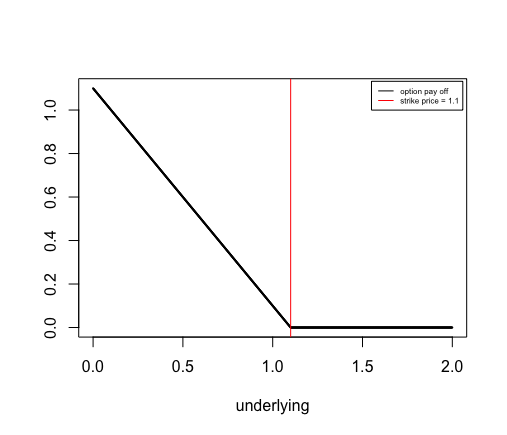
\includegraphics[scale=0.5]{PlotOption.png}
  \label{fig:PlotOption}
  \caption{Auszahlung einer Put Option mit strike 1.1}
\end{figure}

Für eine europäische Option, bei welcher der Ausübungszeitpunkt bekannt ist, ist die Bewertung der Option im Black-Scholes Moell in geschlossener Form möglich. Diese ist in \cite{Hull} auf S.313 zu finden. Weiters führt Hull auch eine Skizze zur Herleitung an.\\
Die Schwierigkeit bei der Bewertung amerikanischer Optionen besteht darin, dass der Ausübungszeitpunkt nicht bekannt ist. Der K"aufer der Option muss also zu jedem Zeitpunkt abwägen, ob die Option ausgeübt werden soll, oder ob die Alternative d.h. die Beibehaltung der Option und eine spätere Aus"ubung sinvoller ist. 
Der Longstaff Schwartz Algorithmus besteht im Wesentlichen aus zwei Teilen. Zum einen, der grundlegenden Simulation von einer ausreichenden Zahl an Preis Trajektorien des \textit{underlying} über die Zeit. Und dem Algorithmus selbst wobei iterativ zu jedem Zeitpunkt der Auszahlungsbetrag bei Aus"ubung und der Erwartungswert bei Beibehaltung verglichen wird. Dieser Erwartungswert berechnet sich durch Schätzen eines linearen Modells der \textit{stock} prices auf die ex-post Auszahlungen mittels der kleinste Quadrate Methode. Davon is auch der Name  Least Squares Monte Carlo (LSM) des Algorithmus abgeleitet.\footnote{vgl. \cite[S.114]{schwartz2001}} 


\subsection{Illustratives Beispiel}

Folgendes Beispiel soll helfen den Least Squares Monte Carlo (LSM) Algorithmus zu veranschaulichen. \\
Um die Bewertung amerikanischer Optionen zu veranschaulichen, ist es sinnvoll, zunächst sog. \glqq Bermuda Optionen\grqq zu betrachten. Dieser Typ von Optionen, lässt eine Ausübung am Laufzeit Ende, wie bei der europäischen Option zu, als auch an festgelegten Ausübungszeitpunkten über die Laufzeit hinweg (z.B. zum Monatsende oder Jahresende). Weil dieser Optionstyp sowohl Charakteristika einer europäischen Option als auch einer amerikanischen Option hinsichtlich der Ausübung vereint, nennt man sie auch „Bermuda-Optionen“. \footnote{\textit{Bermuda} bezieht sich auf die geographische Lage der Bermuda Inseln zwischen Amerika und Europa}\footnote{vgl. \cite{Fries}}\\
Der aktuelle Preis sei normiert und liegt bei 1. Der Strike Preis (i.e. Aus"ubungspreis der Option) bei $K=1.1$. Man gehe weiters davon aus, dass die Option j"ahrlich ausge"ubt werden kann und eine Laufzeit von 4 Jahren hat. Der risikofreie Zinssatz $r$ betrage 6\%\\
Im ersten Schritt werden sog. Pfade simuliert. Hierbei handelt es sich um den Preis des Underlyings. Die Anzahl der Pfade ist dabei beliebig.\footnote{Wie bei Monte-Carlo simulationen "ublich, betimmt allerdings die Zahl der Simulationen die Robustheit der Schätzung} Um das Beispiel "ubersichtlich zu gestalten, werden wir hier nur 10 Pfade simulieren. Jeder Pfad (notiert als Vektor mit 5 Elementen), besteht aus dem konstanten Startpreis (zum ZP $t=0$) und 4 simulierten Preisen.\\


Tabelle \ref{tab:M} zeigt die Matrix der Simulationen des Underlyings. Ein Plot der Pfade findet sich in Abbildung \ref{fig:pfade}.





\begin{table}[H] \centering 
  \caption{Simulationsmatrix} 
  \label{tab:M} 
\begin{tabular}{@{\extracolsep{5pt}} cccccc} 
\\[-1.8ex]\hline 
\hline \\[-1.8ex] 
 & t0 & t1 & t2 & t3 & t4 \\ 
\hline \\[-1.8ex] 
1 & $1$ & $0.832$ & $1.199$ & $0.879$ & $1.007$ \\ 
2 & $1$ & $0.931$ & $1.039$ & $0.973$ & $0.885$ \\ 
3 & $1$ & $1.091$ & $1.588$ & $1.280$ & $1.549$ \\ 
4 & $1$ & $1.021$ & $1.054$ & $0.836$ & $1.099$ \\ 
5 & $1$ & $1.039$ & $0.872$ & $0.685$ & $0.931$ \\ 
6 & $1$ & $1.515$ & $2.051$ & $1.545$ & $1.751$ \\ 
7 & $1$ & $1.138$ & $1.288$ & $1.539$ & $1.705$ \\ 
8 & $1$ & $0.620$ & $0.030$ & $0.077$ & $0.058$ \\ 
9 & $1$ & $0.794$ & $1.004$ & $0.663$ & $0.571$ \\ 
10 & $1$ & $0.866$ & $0.724$ & $1.101$ & $0.986$ \\ 
\hline \\[-1.8ex] 
\end{tabular} 
\end{table} 


\begin{figure}[H]

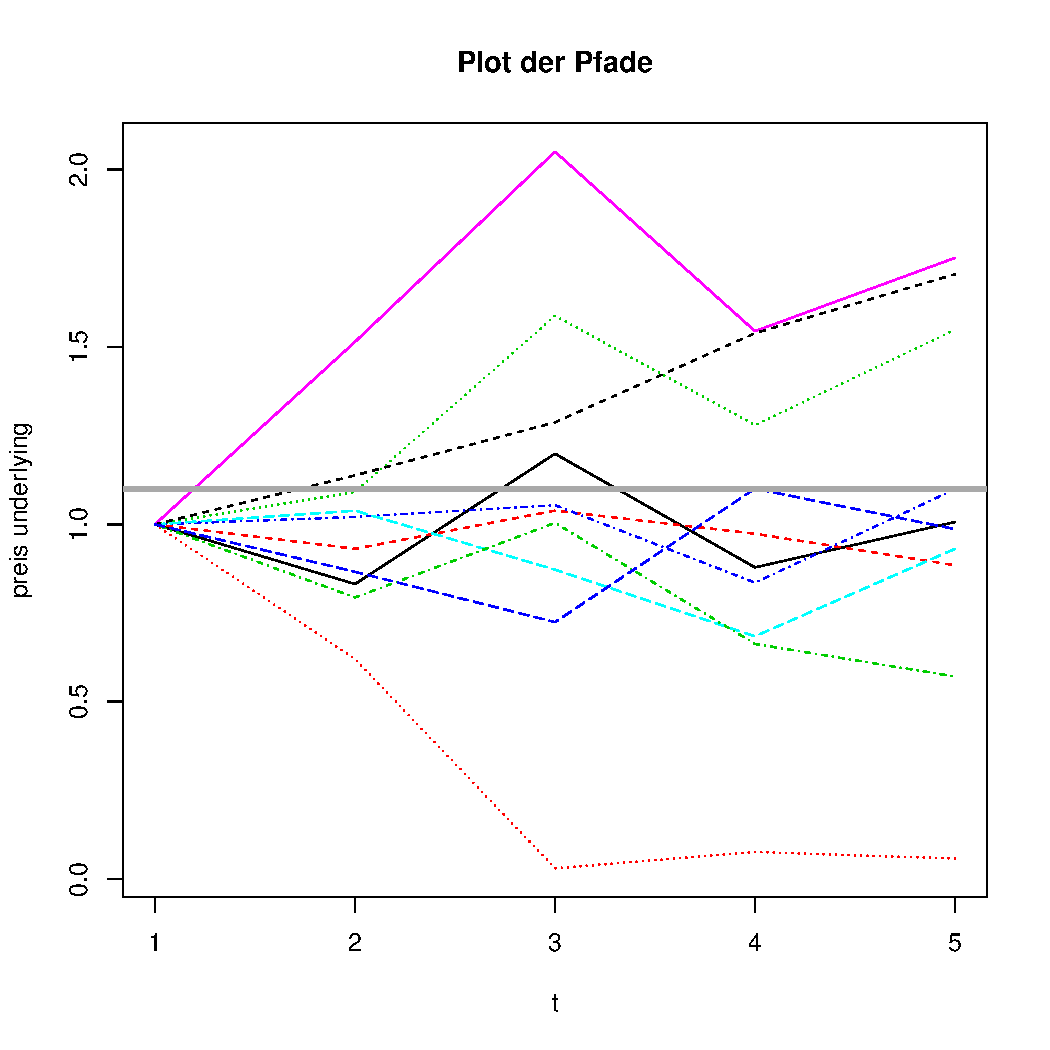
\includegraphics[width=\maxwidth]{figure/unnamed-chunk-3-1} 

\label{fig:pfade}
\caption{Plot der simulierten 10 Pfade; Strikepreis in grau eingezeichnet}
\end{figure}

LSM ist ein (in Bezug auf die Zeit) rekursiver Algorithmus \cite[S.116]{schwartz2001}. D.h. wir beginnen die Iterationen mit dem Laufzeitende (hier t=4). Die Auszahlungen am Laufzeitende f"ur die Simulationen einer Put Option berechnet sich mit $a_T=max\left(K-x_T, 0\right)$ (wir notieren die einzelnen Auszalungen für die jeweilige Simulation $i=1,...,n$ als $a_{i,t}$ und weiters die Spalten der Auszahlungsmatrix $A=\left( \begin{array}{ccc}
\ddots & \vdots & \text{\reflectbox{$\ddots$}} \\
\dots & a_{it} & \dots \\
\text{\reflectbox{$\ddots$}}& \vdots & \ddots \end{array} \right)$ im jeweiligen Zeitpunkt $t=1,...,T$ als Vektoren $a_{\cdot,t}$, dabei wird der Einfachheit halber auf den Punkt der die Zeilen repräsentiert verzichtet). Die Vektoren\footnote{Spalten der Matrix $X=\left( \begin{array}{ccc}
\ddots & \vdots & \text{\reflectbox{$\ddots$}} \\
\dots & x_{it}^z & \dots \\
\text{\reflectbox{$\ddots$}}& \vdots & \ddots \end{array} \right)$} $x_{\cdot,t}$ die die Preise des Underlyings mit $t\in\{1,...,T\}$) repräsentieren folgen der gleichen Notation.


\begin{table}[H] \centering 
  \caption{Auszahlungsmatrix zum Zeitpunkt t=4} 
  \label{tab:t4} 
\begin{tabular}{@{\extracolsep{5pt}} cccccc} 
\\[-1.8ex]\hline 
\hline \\[-1.8ex] 
 & t0 & t1 & t2 & t3 & t4 \\ 
\hline \\[-1.8ex] 
1 & $$ & $$ & $$ & $$ & $0.093$ \\ 
2 & $$ & $$ & $$ & $$ & $0.215$ \\ 
3 & $$ & $$ & $$ & $$ & $0$ \\ 
4 & $$ & $$ & $$ & $$ & $0.001$ \\ 
5 & $$ & $$ & $$ & $$ & $0.169$ \\ 
6 & $$ & $$ & $$ & $$ & $0$ \\ 
7 & $$ & $$ & $$ & $$ & $0$ \\ 
8 & $$ & $$ & $$ & $$ & $1.042$ \\ 
9 & $$ & $$ & $$ & $$ & $0.529$ \\ 
10 & $$ & $$ & $$ & $$ & $0.114$ \\ 
\hline \\[-1.8ex] 
\end{tabular} 
\end{table} 


Nun gilt es die erwarteten Auszahlungen der Option in $t=4$ zu sch"atzen, ausgehend von den simulierten Preisen des Underlyings zum Zeitpunkt $t=3$. Um den Zeitwert der Auszahlungen zu ber"ucksichtigen, werden die Auszahlungen um eine Periode abgezinst.\footnote{wobei eine Periode einem Jahr entspricht} 
Wir erhalten also die Spalte einer neuen Matrix $A^z=\left( \begin{array}{ccc}
\ddots & \vdots & \text{\reflectbox{$\ddots$}} \\
\dots & a_{it}^z & \dots \\
\text{\reflectbox{$\ddots$}}& \vdots & \ddots \end{array} \right)$, die zum ersten Schritt ausschließlich die Eintragungen $a_4^z$ beinhaltet.
\[a_t^z=\exp(-r)\cdot a_t\] 
Um den Erwartungswert in Abh"angigkeit vom simulierten Underlying zu sch"atzen, verwenden wir das folgende lineare Modell:

$$ a_{j,t}^z=\beta_0+\beta_1 a_{j,t-1} + \beta_2 a_{j,t-1}^2 +u_j\ \forall\ j:\ x_{j,t-1}>K$$.\footnote{Es werden nur die Pfade verwendet, bei denen die Option in $t=3$ ausge"ubt werden w"urde, also bei denen es in $t=3$ einen Cash Flow gibt (m.a.W. \textit{in the money}).} F"ur den ersten Regressionsschritt ist $t=4$ in unserem Beispiel.\\
In der Tabelle \ref{tab:R3} sind die Daten f"ur die Regression zusammengefasst. 


\begin{table}[H] \centering 
  \caption{Datenmatrix zur Regressionschritt 1} 
  \label{tab:R3} 
\begin{tabular}{@{\extracolsep{5pt}} ccc} 
\\[-1.8ex]\hline 
\hline \\[-1.8ex] 
 & Y & X \\ 
\hline \\[-1.8ex] 
1 & $0.088$ & $0.221$ \\ 
2 & $0.203$ & $0.127$ \\ 
4 & $0.001$ & $0.264$ \\ 
5 & $0.159$ & $0.415$ \\ 
8 & $0.981$ & $1.023$ \\ 
9 & $0.498$ & $0.437$ \\ 
\hline \\[-1.8ex] 
\end{tabular} 
\end{table} 



Wir betrachten nun also die Werte des Sch"atzers und vergleichen diese mit den Werten, wenn wir die Option schon in $t=3$ aus"uben w"urden.


\begin{table}[H] \centering 
  \caption{Vergleiche Ausueben vs. Beibehalten im ZP t=3} 
  \label{tab:AB} 
\begin{tabular}{@{\extracolsep{5pt}} ccc} 
\\[-1.8ex]\hline 
\hline \\[-1.8ex] 
 & beibehalten & ausueben \\ 
\hline \\[-1.8ex] 
1 & $0.121$ & $0.221$ \\ 
2 & $0.023$ & $0.127$ \\ 
4 & $0.166$ & $0.264$ \\ 
5 & $0.322$ & $0.415$ \\ 
8 & $0.953$ & $1.023$ \\ 
9 & $0.345$ & $0.437$ \\ 
\hline \\[-1.8ex] 
\end{tabular} 
\end{table} 


Beim Vergleich der Werte in Tabelle \ref{tab:AB} sollte jeweils in t=3 ausge"ubt werden, wenn Aus"uben$>$Beibehalten und umgekehrt. Es f"allt auf, dass zu t=3 in allen Pfaden, die \textit{in the money} sind (also 1,2,4,5,8 und 9) ausge"ubt werden soll. An diesen Pfaden "ubernehmen wir den Wert in die Auszahlungsmatrix $A$ und setzen den Wert in t=4 auf null, weil die amerikanische Option nur einmal ausge"ubt werden kann.


\begin{table}[H] \centering 
  \caption{Auszahlungsmatrix zum Zeitpunkt t=3} 
  \label{tab:A3} 
\begin{tabular}{@{\extracolsep{5pt}} cccccc} 
\\[-1.8ex]\hline 
\hline \\[-1.8ex] 
 & t0 & t1 & t2 & t3 & t4 \\ 
\hline \\[-1.8ex] 
1 & $$ & $$ & $$ & $0.221$ & $0$ \\ 
2 & $$ & $$ & $$ & $0.127$ & $0$ \\ 
3 & $$ & $$ & $$ & $0$ & $0$ \\ 
4 & $$ & $$ & $$ & $0.264$ & $0$ \\ 
5 & $$ & $$ & $$ & $0.415$ & $0$ \\ 
6 & $$ & $$ & $$ & $0$ & $0$ \\ 
7 & $$ & $$ & $$ & $0$ & $0$ \\ 
8 & $$ & $$ & $$ & $1.023$ & $0$ \\ 
9 & $$ & $$ & $$ & $0.437$ & $0$ \\ 
10 & $$ & $$ & $$ & $0$ & $0.114$ \\ 
\hline \\[-1.8ex] 
\end{tabular} 
\end{table} 


Nun modellieren wir eine lineare Regression wie oben mit den entsprechenden Auszahlungen zu $t=2$ als X. Y sei der vorausgegangene Wert der Option bei Aus"ubung, abgezinst auf den Zeitpunkt $t$.\footnote{also die Werte $a_{j,t+1},\ \forall\ j=i\ \text{if}\ x_{i,t}>K$} Tabelle \ref{tab:R2} zeigt wiederum welche Werte für die Regression im Regressionsschritt 2 verwendet wurden und Tabelle \ref{tab:AB2} zeigt die den Vergleich zwischen Schätzer und \textit{pay offs}.


\begin{table}[H] \centering 
  \caption{Datenmatrix zur Regressionsschritt 2} 
  \label{tab:R2} 
\begin{tabular}{@{\extracolsep{5pt}} ccc} 
\\[-1.8ex]\hline 
\hline \\[-1.8ex] 
 & Y & X \\ 
\hline \\[-1.8ex] 
2 & $0.119$ & $0.061$ \\ 
4 & $0.249$ & $0.046$ \\ 
5 & $0.391$ & $0.228$ \\ 
8 & $0.964$ & $1.070$ \\ 
9 & $0.412$ & $0.096$ \\ 
10 & $0.101$ & $0.376$ \\ 
\hline \\[-1.8ex] 
\end{tabular} 
\end{table} 

\begin{table}[H] \centering 
  \caption{Vergleiche Ausueben vs. Beibehalten im ZP t=2} 
  \label{tab:AB2} 
\begin{tabular}{@{\extracolsep{5pt}} ccc} 
\\[-1.8ex]\hline 
\hline \\[-1.8ex] 
 & beibehalten & ausueben \\ 
\hline \\[-1.8ex] 
2 & $0.203$ & $0.061$ \\ 
4 & $0.192$ & $0.046$ \\ 
5 & $0.315$ & $0.228$ \\ 
8 & $0.884$ & $1.070$ \\ 
9 & $0.226$ & $0.096$ \\ 
10 & $0.415$ & $0.376$ \\ 
\hline \\[-1.8ex] 
\end{tabular} 
\end{table} 


Im ZP $t=2$ wird nur im Pfad 8 ausge"ubt, ansonsten wird beibehalten. Das f"uhrt zur Auszahlungsmatrix Tabelle \ref{tab:A2}.


\begin{table}[H] \centering 
  \caption{Auszahlungsmatrix zum Zeitpunkt t=2} 
  \label{tab:A2} 
\begin{tabular}{@{\extracolsep{5pt}} cccccc} 
\\[-1.8ex]\hline 
\hline \\[-1.8ex] 
 & t0 & t1 & t2 & t3 & t4 \\ 
\hline \\[-1.8ex] 
1 & $$ & $$ & $0$ & $0.221$ & $0$ \\ 
2 & $$ & $$ & $0$ & $0.127$ & $0$ \\ 
3 & $$ & $$ & $0$ & $0$ & $0$ \\ 
4 & $$ & $$ & $0$ & $0.264$ & $0$ \\ 
5 & $$ & $$ & $0$ & $0.415$ & $0$ \\ 
6 & $$ & $$ & $0$ & $0$ & $0$ \\ 
7 & $$ & $$ & $0$ & $0$ & $0$ \\ 
8 & $$ & $$ & $1.070$ & $0$ & $0$ \\ 
9 & $$ & $$ & $0$ & $0.437$ & $0$ \\ 
10 & $$ & $$ & $0$ & $0$ & $0.114$ \\ 
\hline \\[-1.8ex] 
\end{tabular} 
\end{table} 


F"ur den letzten Schritt $t=1$ verfahren wir genauso (s. Tabelle \ref{tab:A11}). 


\begin{table}[H] \centering 
  \caption{Auszahlungsmatrix im Zeitpunkt t=1} 
  \label{tab:A11} 
\begin{tabular}{@{\extracolsep{5pt}} cccccc} 
\\[-1.8ex]\hline 
\hline \\[-1.8ex] 
 & t0 & t1 & t2 & t3 & t4 \\ 
\hline \\[-1.8ex] 
1 & $$ & $0$ & $0$ & $0.221$ & $0$ \\ 
2 & $$ & $0$ & $0$ & $0.127$ & $0$ \\ 
3 & $$ & $0.009$ & $0$ & $0$ & $0$ \\ 
4 & $$ & $0$ & $0$ & $0.264$ & $0$ \\ 
5 & $$ & $0$ & $0$ & $0.415$ & $0$ \\ 
6 & $$ & $0$ & $0$ & $0$ & $0$ \\ 
7 & $$ & $0$ & $0$ & $0$ & $0$ \\ 
8 & $$ & $0$ & $1.070$ & $0$ & $0$ \\ 
9 & $$ & $0$ & $0$ & $0.437$ & $0$ \\ 
10 & $$ & $0$ & $0$ & $0$ & $0.114$ \\ 
\hline \\[-1.8ex] 
\end{tabular} 
\end{table} 


Zum ZP $t=0$ kann die Option nicht ausge"ubt werden, weshalb ZP $t=0$ irrelevant ist. Die Auszahlungen der Option werden jeweils auf den Zeitpunkt t=0 diskontiert (s. Tabelle \ref{tab:A99}).


\begin{table}[H] \centering 
  \caption{Diskontierte Auszahlungsmatrix} 
  \label{tab:A99} 
\begin{tabular}{@{\extracolsep{5pt}} ccccc} 
\\[-1.8ex]\hline 
\hline \\[-1.8ex] 
 & t1 & t2 & t3 & t4 \\ 
\hline \\[-1.8ex] 
1 & $0$ & $0$ & $0.185$ & $0$ \\ 
2 & $0$ & $0$ & $0.106$ & $0$ \\ 
3 & $0.008$ & $0$ & $0$ & $0$ \\ 
4 & $0$ & $0$ & $0.221$ & $0$ \\ 
5 & $0$ & $0$ & $0.347$ & $0$ \\ 
6 & $0$ & $0$ & $0$ & $0$ \\ 
7 & $0$ & $0$ & $0$ & $0$ \\ 
8 & $0$ & $0.949$ & $0$ & $0$ \\ 
9 & $0$ & $0$ & $0.365$ & $0$ \\ 
10 & $0$ & $0$ & $0$ & $0.089$ \\ 
\hline \\[-1.8ex] 
\end{tabular} 
\end{table} 


Der Wert der Option berechnet sich durch Mitteln der diskontierten Auszahlungen.
In diesem Beispiel:
0.173
.

\section{Anwendungsbeispiel}

Angenommen man möchte nun LSM auf eine amerikanische Put Option anwenden. Zum Stock (dem Underlying der Option) sei der Mittelwert und die Varianz bekannt. Wir gehen in diesem Fall von einer Laufzeit von einem Jahr und einem strike price von 1.1 aus. Innerhalb dieses Jahres, kann die Option zu jedem Handelstag ausgeübt werden. Man gehe davon aus, dass ein Stock zum ersten B"orsentag mit dem Preis $S_0$ startet. Hier sei $S_0=1$. Der risikofreie, jährliche Zinssatz $r$ betrage 1\%. Zur Bepreisung dieser Option müssen wir nun in einem ersten Schritt ausreichend viele Trajektorien über den Zeitraum der Laufzeit hinweg simulieren. Anschließend lässt sich LSM auf diese Simulation anwenden. 

\begin{mybem}
LSM ist eine Heuristik ausschließlich gedacht zur Ermittlung eines fairen Preises einer Option, nicht zur Berechnung des optimalen Ausübungs-zeitpunktes.
\end{mybem}

\subsection{Simulation im Black-Scholes Modell}

F"ur diese Arbeit sollen die Aktienpreise anhand des Black-Scholes Modells für ein Jahr simuliert werden. Man gehe von einem B"orsenjahr aus, d.h. für 2019 252 Handelstage.\footnote{\cite[]{boersewien2019}}\\
Für gegebene Volatilität $\sigma$ ist der (risikoneutrale) Aktienpreisprozess durch die geometrische Brownsche Bewegung
$$S^*(t)=S_0\ \exp\left\{  \left(r-\frac{\sigma^2}{2}\right)t + \sigma W_t\right\}$$
modelliert, wobei $W_t$ den Wiener Prozess bezeichnet.\\
In der Abbildung \ref{fig:pfade252} ist exemplarisch ein Plot mit 10 Pfaden angeführt.


\begin{figure}[H]

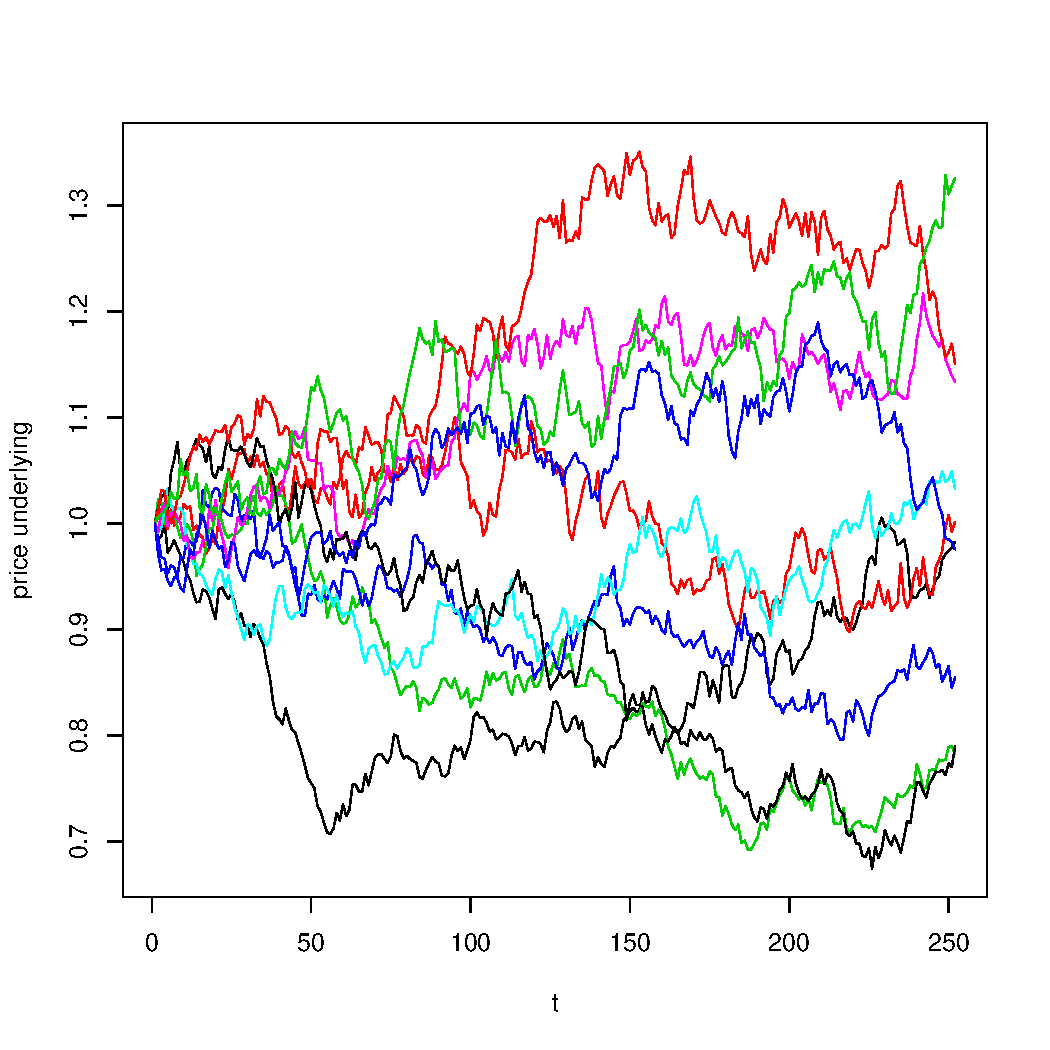
\includegraphics[width=\maxwidth]{figure/unnamed-chunk-14-1} 

\caption{Plot einer Simulation von 10 Pfaden "uber 252 Tage}
\label{fig:pfade252}
\end{figure}

\begin{mybem}
Um die Korrektheit der Implementierung zu überprüfen, soll nun veranschaulicht werden, dass der simulierte Prozess näherungsweise ein Martingal darstellt. Angenommen ein zeitdiskreter Prozess $(X_t)_{t\geq 1}$ sei integrierbar und adaptiert (d.h. $\mathcal{F}_n$ meßbar f"ur alle $n \in \mathbb{N}$, wobei $\mathcal{F}_n$ eine Filtration zum ZP $n$). Der Prozess ist genau dann ein Martingal, wenn folgende Martingaleigenschaft erfüllt ist:
\[ \mathbb{E}\left[X_{t+1}| \mathcal{F}_t\right]=X_t \ \ f.s.\ \ \forall t \in \mathbb{N}\]
Für unseren simulierten Fall würde das bedeuten, dass der Prozess einen konstanten, diskontierten Erwartungswert hat, was es zu "uberpr"ufen gilt. Im Folgenden wird also der Erwartungswert für alle $t$ durch das arithmetische Mittel geschätzt. Um validere Ergebnisse zu erhalten, sollen nun 1000 Pfade simuliert werden (Plot im Appendix Abbildung \ref{100P}). Der Plot in Abbildung \ref{EWfig} zeigt die Sch"atzer für alle Beobachtungszeitpunkte. 
\end{mybem}

\begin{figure}[H]

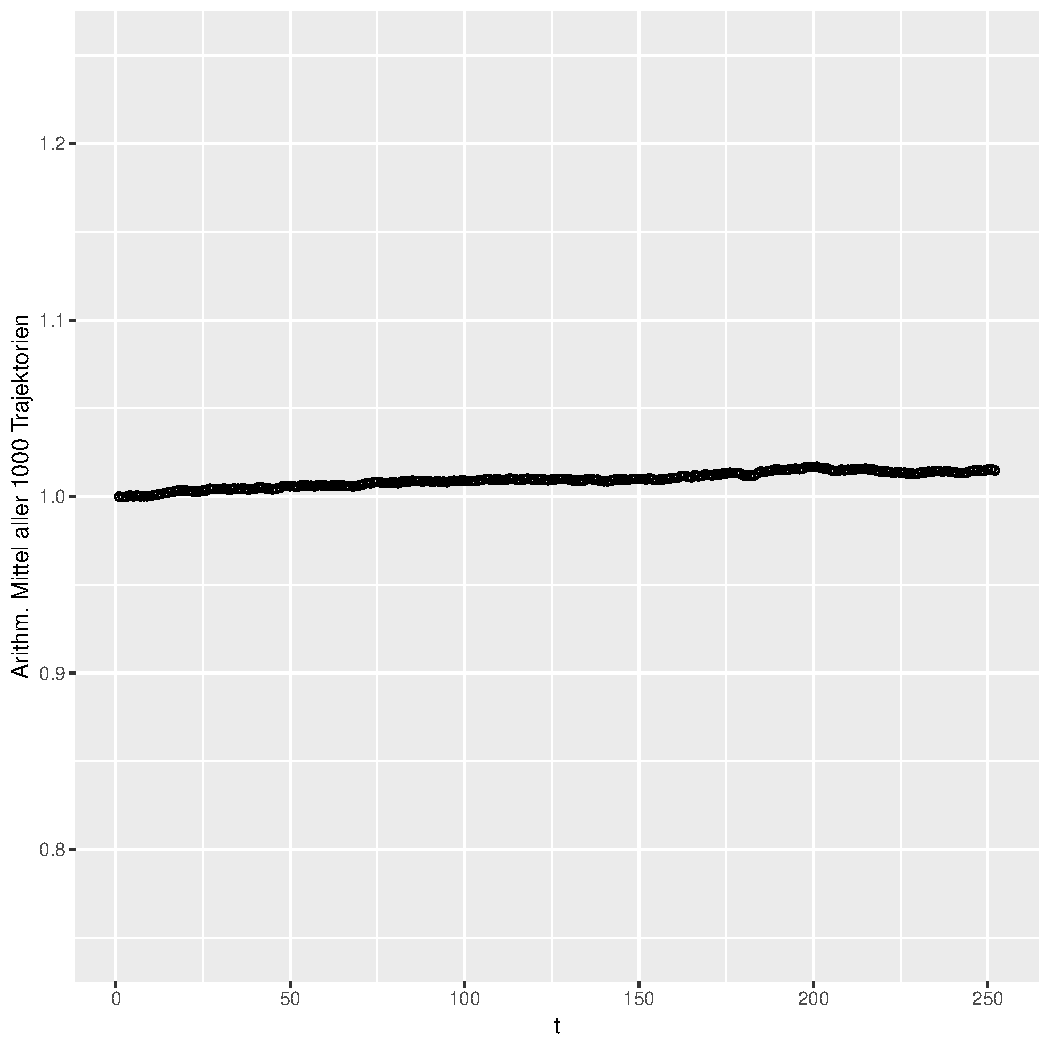
\includegraphics[width=\maxwidth]{figure/unnamed-chunk-15-1} 

\caption{Plot der gesch"atzten Erwartungswerte (d.h. arithm. Mittel) für den Prozess mit 1000 Pfaden}
\label{EWfig}
\end{figure}

Der Plot der Mittel in Abbildung \ref{EWfig} st"utzt die Annahme, dass der Erwartungswert für alle $t \in \mathbb{N}$ konstant ist. Man kann also davon ausgehen, dass es sich bei dem simulierten Prozess um ein Martingal handelt. 

\subsection{Anwendung von LSM auf simulierte Preise}

Nun wollen wir LSM auf die simulierten Preise anwenden um einen fairen Preis für die Option zu berechnen. Dazu soll die Funktion \textit{LSM()} (s. Appendix) dienen, welche die simulierte Matrix als Argument übernimmt. 


\ \\
Der resultierende Wert beträgt  
0.129
.

\ \\
Wir haben im einführenden Beispiel und für den LSM Algorithmus oben ein Polynom 2. Grades für das lineare Modell gewählt. Nun stellt sich die Frage: Wie unterschiedlich sind die Ergebnisse für verschiedene Modelle?\\
Ich möchte im Folgenden nur eine Übersicht über einige wenige Modelle geben. Interessant ist der Vergleich mit folgenden Modellen:

\begin{itemize}
\item dem einfachen Mittelwert - Mittelwertmodell ($ a_{j,t}^z=\beta_0+u_j $)
\item einem einfachen linearen Modell ($ a_{j,t}^z=\beta_0+\beta_1 a_{j,t-1}+u_j $)
\item einem linearen Modell ohne intercept ($ a_{j,t}^z=\beta_1 a_{j,t-1}+u_j $)
\item einem linearen Modell mit einem Polynom dritten Grades ($ a_{j,t}^z=\beta_0+\beta_1 a_{j,t-1} + \beta_2 a_{j,t-1}^2 + \beta_2 a_{j,t-1}^3  +u_j $)
\item und einem Modell mit einem Polynom 10ten Grades. ($ a_{j,t}^z=\beta_0+\beta_1 a_{j,t-1} + \beta_2 a_{j,t-1}^2 + ... + \beta_2 a_{j,t-1}^10  +u_j $)
\end{itemize}

\begin{mybem}
Diese Modelle sind willkürlich gewählt und sollen dem Leser nur einen Überblick vermitteln.
\end{mybem}





% Table created by stargazer v.5.2.2 by Marek Hlavac, Harvard University. E-mail: hlavac at fas.harvard.edu
% Date and time: Mo, Apr 22, 2019 - 18:11:20
\begin{table}[!htbp] \centering 
  \caption{Übersicht der simulierten Optionswerte auf Grundlage unterschiedlicher Modelle} 
  \label{} 
\begin{tabular}{@{\extracolsep{5pt}} ccc} 
\\[-1.8ex]\hline 
\hline \\[-1.8ex] 
 & Modell & Optionswert \\ 
\hline \\[-1.8ex] 
1 & Mittelwertmodell & $0.11459$ \\ 
2 & linear ohne intercept & $0.10017$ \\ 
3 & einfach linear & $0.12883$ \\ 
4 & Polynom 2 & $0.12883$ \\ 
5 & Polynom 3 & $0.12883$ \\ 
6 & Polynom 10 & $0.12883$ \\ 
\hline \\[-1.8ex] 
\end{tabular} 
\end{table} 


Wir beobachten, dass die Optionbewertungen für die linearen Modelle (ausschließlich dem linearen Modell ohne intercept) identisch sind. Der Schluss liegt nahe, dass die Information der simulierten Werte ausreicht, um selbst mit dem einfachen linearen Modell an den selben Zeitpunkten auszuüben, wie auch bei den koplexeren Modellen. Das Mittelwertmodell hingegen lässt den Algorithmus an deutlich anderen Zeitpunkten ausüben was wiederum zu anderen Auszahlungen und in weiterer Folge zu einem anderen Optionswert führt. Das Modell ohne intercept ist ein Sonderfall. Zum einen entspricht dieser Ansatz nicht dem Longstaff Schwartz Algorithmus, weil hier nicht mit dem Aktienpreis als erklärender Variable regressiert wird.\footnote{Bei den anderen Basisfunktionen ist es nicht ausschlaggebend ob von der Datenmatrix eine Kontante $K$ für alle Trajektorien subtrahiert wird, weil sich das nur auf den intercept auswirkt. Das Modell ohne intercept ist nicht invariant gegenüber einer solchen Translation.}\\
Weitere interessante Basisfunktionen, wären beispielsweise Modelle aus den Klassen der lognormalen Modelle oder Modellen mit nichtlinearem Zusammenhang.


\section{Fazit}

Ziel dieser Arbeit war es, verschiedene Basisfunktionen im Longstaff Schwartz Algorithmus anzuwenden und die Resultate zu vergleichen. In Punkt 2 konnte für mehrere Beispiele gezeigt werden, dass die Generalisierung der Basisfunktion im Longstaff Schwartz Algorithmus zu einem linearen Modell mit Polynmen höherer Ordnung zu keiner merklichen Veränderungen im simulierten Wert der Option geführt hat. Allerdings stellte sich für zwei Basisfunktionen, die nicht in die Klasse der linearen Modelle mit Intercept fallen heraus, dass sich das Ergebnisse deutlich unterscheiden. Diese Arbeit kann Grundlage sein zur Untersuchung der Auswirkung verschiedener anderer Basisfunktionen auf die Longstaff Schwartz Methode.

\newpage 

\bibliography{SeminararbeitBiBTex}
\bibliographystyle{apalike}



\section*{Appendix}

\begin{figure}[H]

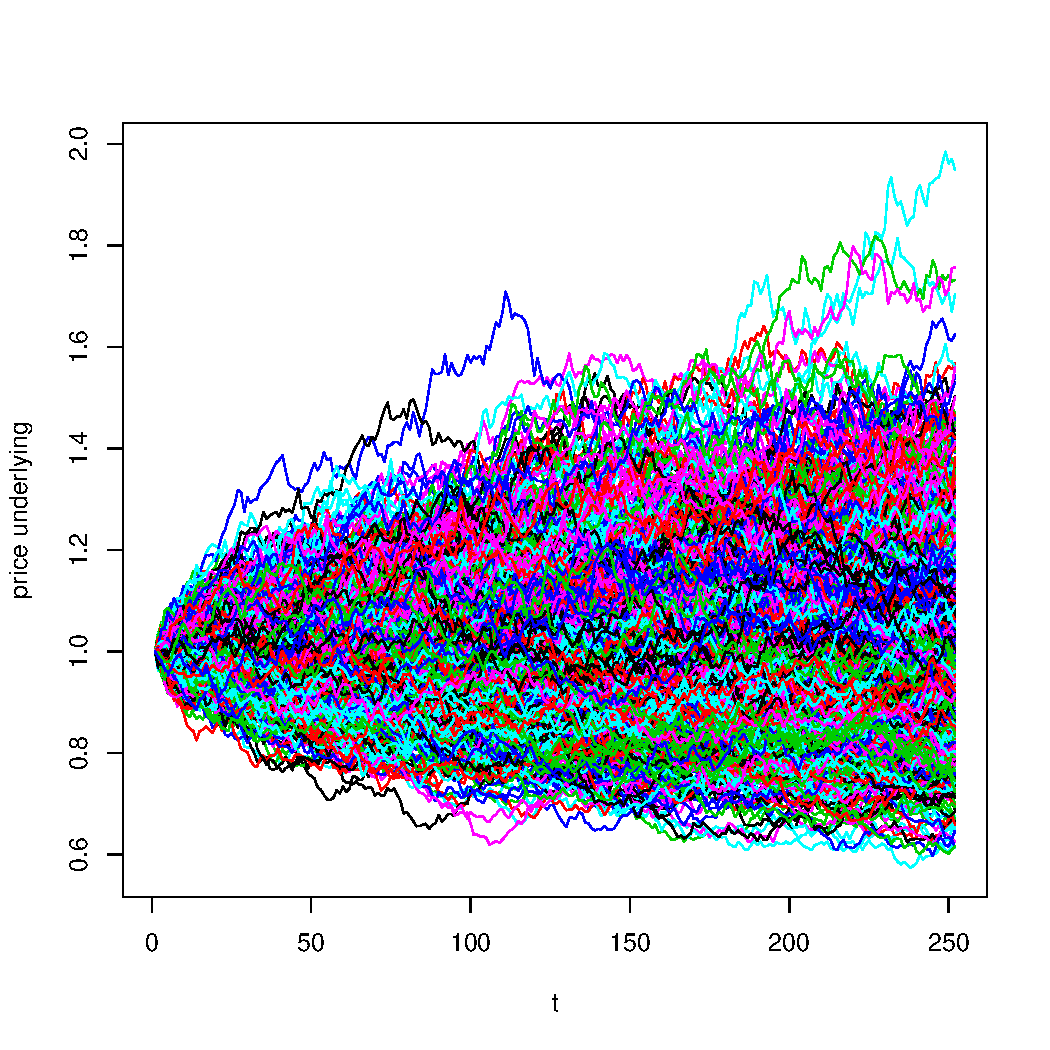
\includegraphics[width=\maxwidth]{figure/unnamed-chunk-20-1} 

\caption{Plot der Simulation mit 1000 Pfaden}
\label{100P}
\end{figure}

Funktion \textit{simMatrix()} um die Matrix der stock Preise zu simulieren.

\begin{kframe}
\begin{alltt}
\hlstd{simMatrix} \hlkwb{<-} \hlkwa{function}\hlstd{(}\hlkwc{S0}\hlstd{=}\hlnum{100}\hlstd{,} \hlkwc{Nsimulations}\hlstd{=}\hlnum{100}\hlstd{,} \hlkwc{r}\hlstd{=}\hlnum{0.01}\hlstd{,}
                      \hlkwc{sigma}\hlstd{=}\hlnum{0.2}\hlstd{,} \hlkwc{se}\hlstd{=}\hlnum{123}\hlstd{)\{}
  \hlcom{# simMatrix is a function, simulating a Matrix of stock}
  \hlcom{# prices for one year. The number of simulations can be}
  \hlcom{# set by the parameter Nsimulations. }
  \hlcom{# The function simulates the Stock prices using the }
  \hlcom{# Black-Scholes Model. The Stock price for t>0 is given}
  \hlcom{# by: S_t = S_0 * exp\{r-sigma^2/2)*t + sigma*W_t\}, where W_t is }
  \hlcom{# a Brownian Motion with mu=0 and variance is the time increment.}
  \hlcom{# Nsimulations ... Number of simulations (int)}
  \hlcom{# S0 ............. Starting value (int)}
  \hlcom{# r .............. risk free interest rate (int)}
  \hlcom{# sigma .......... the parameter sigma for the Black Scholes}
  \hlcom{#                  simulation. }
  \hlcom{# se ............. set seed (int)}

  \hlkwd{set.seed}\hlstd{(se)}
  \hlstd{M} \hlkwb{<-} \hlkwd{matrix}\hlstd{(}\hlnum{NA}\hlstd{,} \hlkwc{nrow}\hlstd{=Nsimulations,} \hlkwc{ncol}\hlstd{=}\hlnum{252}\hlstd{)}
  \hlstd{N} \hlkwb{<-} \hlnum{252}
  \hlkwa{for} \hlstd{(i} \hlkwa{in} \hlnum{1}\hlopt{:}\hlstd{Nsimulations)\{}

    \hlcom{# Brownian Motion}
    \hlstd{m} \hlkwb{<-} \hlnum{0}
    \hlstd{dW} \hlkwb{<-} \hlkwd{rnorm}\hlstd{(}\hlkwc{n}\hlstd{=N,} \hlkwc{mean}\hlstd{=m,} \hlkwc{sd}\hlstd{=}\hlkwd{sqrt}\hlstd{(}\hlnum{1}\hlopt{/}\hlnum{252}\hlstd{))}
    \hlstd{W} \hlkwb{<-} \hlkwd{c}\hlstd{(}\hlnum{0}\hlstd{,} \hlkwd{cumsum}\hlstd{(dW))}

    \hlstd{t} \hlkwb{<-} \hlnum{1}\hlopt{:}\hlstd{N}
    \hlstd{S} \hlkwb{<-} \hlstd{S0}\hlopt{*}\hlkwd{exp}\hlstd{((r}\hlopt{-}\hlstd{(sigma}\hlopt{^}\hlnum{2}\hlstd{)}\hlopt{/}\hlnum{2}\hlstd{)}\hlopt{*}\hlstd{(t}\hlopt{/}\hlnum{252}\hlstd{)}\hlopt{+}\hlstd{sigma}\hlopt{*}\hlstd{W[t}\hlopt{+}\hlnum{1}\hlstd{])}
    \hlstd{M[i,]} \hlkwb{<-} \hlstd{S}
  \hlstd{\}}
  \hlkwd{colnames}\hlstd{(M)} \hlkwb{<-} \hlnum{1}\hlopt{:}\hlnum{252}
  \hlkwd{rownames}\hlstd{(M)} \hlkwb{<-} \hlkwd{paste}\hlstd{(}\hlstr{"sim"}\hlstd{,} \hlnum{1}\hlopt{:}\hlstd{Nsimulations)}
  \hlkwd{return}\hlstd{(M)}
\hlstd{\}}
\end{alltt}
\end{kframe}

Funktion \textit{LSM} um ein LSM Algoritmus auf die Simulation anzuwenden.

\begin{kframe}
\begin{alltt}
\hlstd{LSM} \hlkwb{<-} \hlkwa{function}\hlstd{(}\hlkwc{M}\hlstd{,} \hlkwc{K}\hlstd{=}\hlnum{1.1}\hlstd{,} \hlkwc{r}\hlstd{=}\hlnum{0.06}\hlstd{)\{}
  \hlcom{# This function performs the Least Squares Monte Carlo}
  \hlcom{# algorithm for any simulated matrix M. The output}
  \hlcom{# is the mean of the discounted cash flow of returns }
  \hlcom{# where the option was exercised.}
  \hlcom{# M ... simulated matrix}
  \hlcom{# K ... strike price}
  \hlcom{# r ... interest rate}
  \hlstd{T} \hlkwb{<-} \hlkwd{ncol}\hlstd{(M)}
  \hlstd{t} \hlkwb{<-} \hlstd{T}\hlopt{-}\hlnum{1}
  \hlstd{N} \hlkwb{<-} \hlkwd{nrow}\hlstd{(M)}
  \hlstd{Ai} \hlkwb{<-} \hlkwd{matrix}\hlstd{(}\hlnum{0}\hlstd{,} \hlkwc{nrow}\hlstd{=N,} \hlkwc{ncol}\hlstd{=T)}
  \hlkwd{lapply}\hlstd{(M[,t}\hlopt{+}\hlnum{1}\hlstd{],}\hlkwa{function}\hlstd{(}\hlkwc{x}\hlstd{)} \hlkwd{max}\hlstd{(K}\hlopt{-}\hlstd{x,}\hlnum{0}\hlstd{))}  \hlopt \hlstd{unlist} \hlkwb{->} \hlstd{Ai[,t}\hlopt{+}\hlnum{1}\hlstd{]}

  \hlkwa{for} \hlstd{(t} \hlkwa{in} \hlstd{(T}\hlopt{-}\hlnum{1}\hlstd{)}\hlopt{:}\hlnum{2}\hlstd{)\{}
    \hlkwd{lapply}\hlstd{(M[,t],}\hlkwa{function}\hlstd{(}\hlkwc{x}\hlstd{)} \hlkwd{max}\hlstd{(K}\hlopt{-}\hlstd{x,}\hlnum{0}\hlstd{))}  \hlopt \hlstd{unlist} \hlopt
      \hlkwd{Filter}\hlstd{(}\hlkwc{f}\hlstd{=}\hlkwa{function}\hlstd{(}\hlkwc{x}\hlstd{) x}\hlopt{!=}\hlnum{0}\hlstd{)}\hlkwb{->} \hlstd{im}
    \hlkwd{names}\hlstd{(im)} \hlopt \hlkwd{as.numeric}\hlstd{()} \hlkwb{->} \hlstd{ind}
    \hlcom{# discounting}
    \hlstd{Y} \hlkwb{<-} \hlkwd{rep}\hlstd{(}\hlnum{0}\hlstd{,}\hlkwd{length}\hlstd{(ind))}
    \hlkwa{for} \hlstd{(i} \hlkwa{in} \hlnum{1}\hlopt{:}\hlstd{(T}\hlopt{-}\hlstd{t))\{}
      \hlstd{Y} \hlkwb{<-} \hlstd{Y}\hlopt{+}\hlkwd{exp}\hlstd{(}\hlopt{-}\hlstd{r}\hlopt{*}\hlstd{i)}\hlopt{*}\hlstd{Ai[ind,t}\hlopt{+}\hlstd{i]}
    \hlstd{\}}
    \hlstd{X} \hlkwb{<-} \hlstd{im}
    \hlstd{lm1} \hlkwb{<-} \hlkwd{lm}\hlstd{(Y}\hlopt{~}\hlstd{X}\hlopt{+}\hlstd{(X}\hlopt{^}\hlnum{2}\hlstd{))}
    \hlstd{f1} \hlkwb{<-} \hlstd{lm1}\hlopt{$}\hlstd{fitted.values}
    \hlcom{# exercise vs keep}
    \hlstd{df} \hlkwb{<-} \hlkwd{data.frame}\hlstd{(}\hlkwc{beibehalten}\hlstd{=f1,} \hlkwc{ausueben}\hlstd{=im)}
    \hlstd{ind2} \hlkwb{<-} \hlkwd{apply}\hlstd{(df,}\hlnum{1}\hlstd{,} \hlkwa{function}\hlstd{(}\hlkwc{x}\hlstd{)} \hlkwd{ifelse}\hlstd{(x[}\hlnum{2}\hlstd{]}\hlopt{>}\hlstd{x[}\hlnum{1}\hlstd{], x[}\hlnum{2}\hlstd{],} \hlnum{0}\hlstd{))}
    \hlstd{Ai[ind,t]} \hlkwb{<-} \hlstd{ind2}
    \hlcom{# set all following to 0}
    \hlstd{Ai[Ai[,t]}\hlopt{!=}\hlnum{0}\hlstd{,(t}\hlopt{+}\hlnum{1}\hlstd{)}\hlopt{:}\hlstd{T]} \hlkwb{<-} \hlnum{0}
  \hlstd{\}}

  \hlstd{Ai} \hlkwb{<-} \hlstd{Ai[,}\hlnum{2}\hlopt{:}\hlstd{T]}
  \hlstd{Y} \hlkwb{<-} \hlkwd{rep}\hlstd{(}\hlnum{0}\hlstd{,N)}
  \hlkwa{for} \hlstd{(i} \hlkwa{in} \hlnum{1}\hlopt{:}\hlstd{(T}\hlopt{-}\hlnum{1}\hlstd{))\{}
    \hlstd{Y} \hlkwb{<-} \hlstd{Y}\hlopt{+}\hlkwd{exp}\hlstd{(}\hlopt{-}\hlstd{r}\hlopt{*}\hlstd{i)}\hlopt{*}\hlstd{Ai[,i]}
  \hlstd{\}}
  \hlkwd{return}\hlstd{(}\hlkwd{mean}\hlstd{(Y))}
\hlstd{\}}
\end{alltt}
\end{kframe}


Der gesamte Code ist in folgendem Git \textit{repository} zu finden:
\url{https://github.com/SebastianKnigge/Praktikum_Seminararbeit}

\end{document}
